\tikzset{every picture/.style={line width=0.75pt}} %set default line width to 0.75pt        

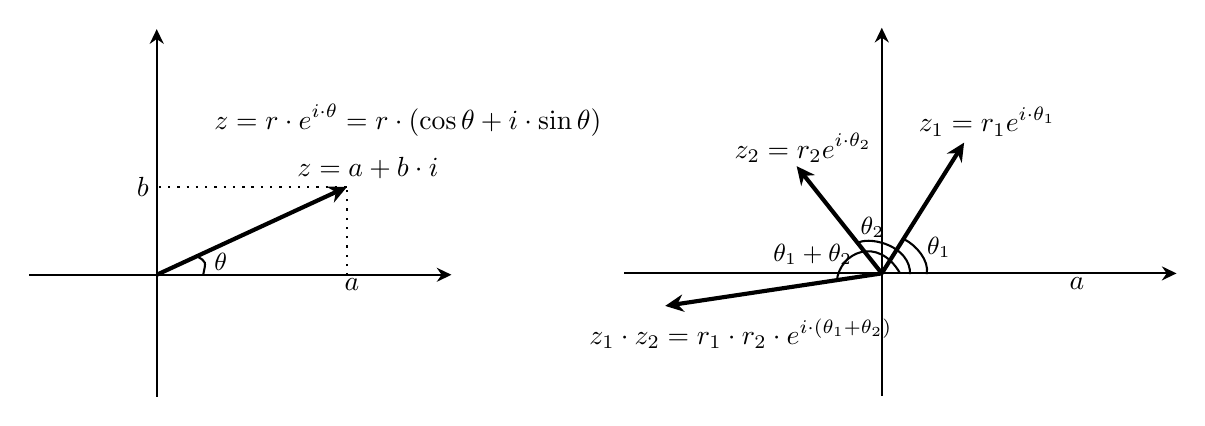
\begin{tikzpicture}[x=0.5pt,y=0.5pt,yscale=-1,xscale=1]
%uncomment if require: \path (0,313); %set diagram left start at 0, and has height of 313

%Straight Lines [id:da8759123208415905] 
\draw [color={rgb, 255:red, 0; green, 0; blue, 0 }  ,draw opacity=1 ][line width=0.75]    (330.52,214.5) -- (28,214.5) ;
\draw [shift={(333.52,214.5)}, rotate = 180] [fill={rgb, 255:red, 0; green, 0; blue, 0 }  ,fill opacity=1 ][line width=0.08]  [draw opacity=0] (10.72,-5.15) -- (0,0) -- (10.72,5.15) -- (7.12,0) -- cycle    ;
%Straight Lines [id:da821272442788836] 
\draw [color={rgb, 255:red, 0; green, 0; blue, 0 }  ,draw opacity=1 ][line width=0.75]    (120.52,40) -- (120.52,303) ;
\draw [shift={(120.52,37)}, rotate = 90] [fill={rgb, 255:red, 0; green, 0; blue, 0 }  ,fill opacity=1 ][line width=0.08]  [draw opacity=0] (10.72,-5.15) -- (0,0) -- (10.72,5.15) -- (7.12,0) -- cycle    ;
%Straight Lines [id:da671644264403058] 
\draw [color={rgb, 255:red, 0; green, 0; blue, 0 }  ,draw opacity=1 ][line width=1.5]    (254.37,152.68) -- (120.52,214.5) ;
\draw [shift={(258,151)}, rotate = 155.21] [fill={rgb, 255:red, 0; green, 0; blue, 0 }  ,fill opacity=1 ][line width=0.08]  [draw opacity=0] (13.4,-6.43) -- (0,0) -- (13.4,6.44) -- (8.9,0) -- cycle    ;
%Straight Lines [id:da23468734573164285] 
\draw [color={rgb, 255:red, 0; green, 0; blue, 0 }  ,draw opacity=1 ][line width=0.75]  [dash pattern={on 0.84pt off 2.51pt}]  (258,215) -- (258,151) ;
%Straight Lines [id:da9615311619238165] 
\draw [color={rgb, 255:red, 0; green, 0; blue, 0 }  ,draw opacity=1 ][line width=0.75]  [dash pattern={on 0.84pt off 2.51pt}]  (122,151) -- (258,151) ;
%Straight Lines [id:da7684706213932966] 
\draw [color={rgb, 255:red, 0; green, 0; blue, 0 }  ,draw opacity=1 ][line width=0.75]    (854.52,213.5) -- (458,213.5) ;
\draw [shift={(857.52,213.5)}, rotate = 180] [fill={rgb, 255:red, 0; green, 0; blue, 0 }  ,fill opacity=1 ][line width=0.08]  [draw opacity=0] (10.72,-5.15) -- (0,0) -- (10.72,5.15) -- (7.12,0) -- cycle    ;
%Straight Lines [id:da6533221507591959] 
\draw [color={rgb, 255:red, 0; green, 0; blue, 0 }  ,draw opacity=1 ][line width=0.75]    (644.52,39) -- (644.52,302) ;
\draw [shift={(644.52,36)}, rotate = 90] [fill={rgb, 255:red, 0; green, 0; blue, 0 }  ,fill opacity=1 ][line width=0.08]  [draw opacity=0] (10.72,-5.15) -- (0,0) -- (10.72,5.15) -- (7.12,0) -- cycle    ;
%Straight Lines [id:da054729749207868106] 
\draw [color={rgb, 255:red, 0; green, 0; blue, 0 }  ,draw opacity=1 ][line width=1.5]    (701.87,122.39) -- (644.52,213.5) ;
\draw [shift={(704,119)}, rotate = 122.19] [fill={rgb, 255:red, 0; green, 0; blue, 0 }  ,fill opacity=1 ][line width=0.08]  [draw opacity=0] (13.4,-6.43) -- (0,0) -- (13.4,6.44) -- (8.9,0) -- cycle    ;
%Straight Lines [id:da37945188035781485] 
\draw [color={rgb, 255:red, 0; green, 0; blue, 0 }  ,draw opacity=1 ][line width=1.5]    (585.49,139.13) -- (644.52,213.5) ;
\draw [shift={(583,136)}, rotate = 51.56] [fill={rgb, 255:red, 0; green, 0; blue, 0 }  ,fill opacity=1 ][line width=0.08]  [draw opacity=0] (13.4,-6.43) -- (0,0) -- (13.4,6.44) -- (8.9,0) -- cycle    ;
%Curve Lines [id:da5454872321119888] 
\draw    (149,201) .. controls (157,205) and (156,205) .. (154,215) ;
%Curve Lines [id:da27173222922396245] 
\draw    (661,189) .. controls (669,193) and (679,204) .. (677,214) ;
%Curve Lines [id:da2426367815741498] 
\draw    (628,191) .. controls (638,187) and (665,194) .. (665,214) ;
%Straight Lines [id:da5276650115271059] 
\draw [color={rgb, 255:red, 0; green, 0; blue, 0 }  ,draw opacity=1 ][line width=1.5]    (491.96,236.41) -- (644.52,213.5) ;
\draw [shift={(488,237)}, rotate = 351.46] [fill={rgb, 255:red, 0; green, 0; blue, 0 }  ,fill opacity=1 ][line width=0.08]  [draw opacity=0] (13.4,-6.43) -- (0,0) -- (13.4,6.44) -- (8.9,0) -- cycle    ;
%Curve Lines [id:da6762459778146103] 
\draw    (612,219) .. controls (614,198) and (642,186) .. (657.76,213.5) ;

% Text Node
\draw (220,127) node [anchor=north west][inner sep=0.75pt]   [align=left] {$\displaystyle z=a+b\cdot i$};
% Text Node
\draw (254,215) node [anchor=north west][inner sep=0.75pt]   [align=left] {$\displaystyle a$};
% Text Node
\draw (104,142) node [anchor=north west][inner sep=0.75pt]   [align=left] {$\displaystyle b$};
% Text Node
\draw (160,197) node [anchor=north west][inner sep=0.75pt]  [font=\small] [align=left] {$\displaystyle \theta $};
% Text Node
\draw (669,91) node [anchor=north west][inner sep=0.75pt]   [align=left] {$\displaystyle z_{1} =r_{1} e^{i\cdot \theta _{1}}$};
% Text Node
\draw (778,214) node [anchor=north west][inner sep=0.75pt]   [align=left] {$\displaystyle a$};
% Text Node
\draw (675,185) node [anchor=north west][inner sep=0.75pt]  [font=\small] [align=left] {$\displaystyle \theta _{1}$};
% Text Node
\draw (431,244) node [anchor=north west][inner sep=0.75pt]   [align=left] {$\displaystyle z_{1} \cdot z_{2} =r_{1} \cdot r_{2} \cdot e^{i\cdot ( \theta _{1} +\theta _{2})}$};
% Text Node
\draw (627,171) node [anchor=north west][inner sep=0.75pt]  [font=\small] [align=left] {$\displaystyle \theta _{2}$};
% Text Node
\draw (160,89) node [anchor=north west][inner sep=0.75pt]   [align=left] {$\displaystyle z=r\cdot e^{i\cdot \theta } =r\cdot (\cos \theta +i\cdot \sin \theta )$};
% Text Node
\draw (536,110) node [anchor=north west][inner sep=0.75pt]   [align=left] {$\displaystyle z_{2} =r_{2} e^{i\cdot \theta _{2}}$};
% Text Node
\draw (564,190) node [anchor=north west][inner sep=0.75pt]  [font=\small] [align=left] {$\displaystyle \theta _{1} +\theta _{2}$};


\end{tikzpicture}

